\chapter{引言}\label{chap:introduction}

\section{本文的研究背景与意义}

云计算改变了人们使用计算资源的方式,人们通过云厂商提供的计算服务能够方便地使用到先进硬件资源,同时云计算具备的弹性、安全等特性也能够为人们节省管理负担。近年来,超大规模数据中心在不断增加。2021年统计数据中~\ref{fig:cloud_compute_scale}, 中国的数据中心数量已超700个,而近年来随AI、物联网、区块链与元宇宙等技术的发展,预计将来超大规模数据中心数量仍然会持续增长,在这一背景下,如何利用数据中心丰富的资源,提高数据中心资源利用率成为云厂商关注的核心问题之一。

\begin{figure}[!htbp]
    \centering
    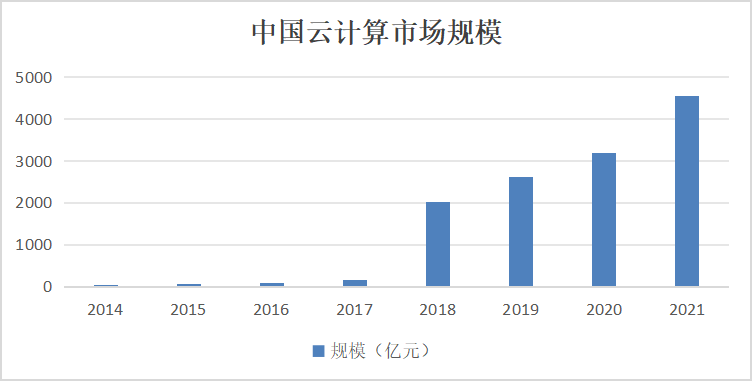
\includegraphics[width=0.80\textwidth]{cloud_compute_scale}
    \bicaption{\quad 中国云计算市场规模增长趋势}{\quad cloud compute scale}
    \label{fig:cloud_compute_scale}
\end{figure}

资源超卖是云厂商提高数据中心资源利用率、增加收入的主要手段之一。超卖主要涉及计算资源与存储资源。CPU是最常见的超卖资源,虚拟化技术允许在一个CPU运行多个虚拟CPU,超卖意味着售出的虚拟CPU资源超过了当前节点上物理核心数量,内存超卖则依赖内存页共享交换机制,但不同于CPU资源超卖,内存的超卖风险较高,因为一旦物理内存耗尽,就会导致系统性能的急剧下降,存储超卖则意味着出售给用户比节点实际存储还要多的存储资源,这通常基于用户一般不会完全使用存储空间的假设,而存储池的设计也能够及时的满足用户的存储需求,网络带宽同样可以进行超卖,这是因为用户在网络的使用存在时间上的不均,同时也依赖一定的网络调控手段来避免网络出现拥塞和劣化。

随虚拟化技术不断进步,从以Xen、KVM技术为核心的虚拟机,到以容器为核心的kubernetes,再到更前沿的ServerLess、FaaS平台,虚拟化技术的提升对用户屏蔽了越来越多的底层细节,使得用户能够越来越专注核心的业务逻辑,而对云厂商而言,则能够提供更细粒度的计算、存储资源。

\begin{figure}[!htbp]
    \centering
    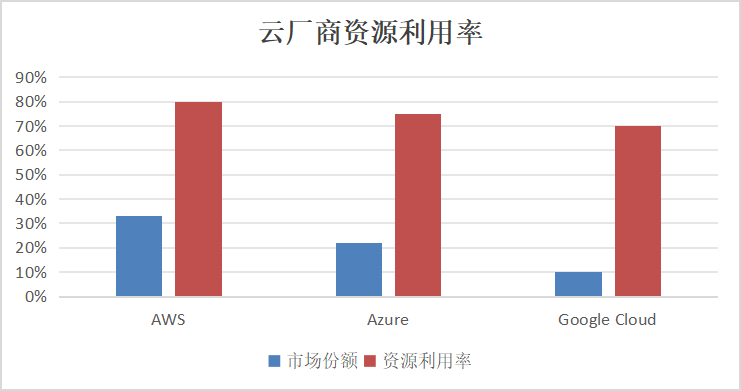
\includegraphics[width=0.80\textwidth]{cloud_compute_utilization}
    \bicaption{\quad 云厂商市场份额及利用率}{\quad cloud compute utilization}
    \label{fig:cloud_compute_utilization}
\end{figure}

细粒度的资源管理意味着更多的超卖机会,然而不恰当的超卖策略会对用户产生较严重影响,同时越上层的虚拟化技术能够提供给用户的信息越少,导致用户难以通过常规的手段去观测或调优。但是如同商品需要提供质量凭证,云厂商也应当为其所出售的云产品提供质量保证,因此云厂商会与用户协商云产品的SLO,用来指定来指定云产品所提供功能的一种期望状态,通常包含每秒请求数量、延迟、服务可用性以及带宽等关键性能指标,并协商在违反SLO是对用户予以补偿。

SLO为用户提供了保证,也意味着SLO的破坏会给用户及云厂商都带来损失,在提升资源利用率与SLO保证中取舍是云厂商需要关注的核心问题之一。实现SLO保证依赖持续的监测与调度机制。可观测性技术是常见的监控机制,其通常为一套数据采集系统,从应用内、运行时及集群获取不同纬度的监控信息,帮助运维人员了解云产品的运行情况。应用内的可观测性机制通常为内嵌的性能监控代码,在应用运行时记录性能信息,并提供API接口以便外部访问,这些指标能够直接反映SLO。运行时的可观测性则从应用运行的上下文中获取有效信息,如内核中对任务使用资源的统计。集群可观测性突出多节点的特征,反映端到端的性能情况,在微服务背景下,集群级别的可观测性机制越来越重要。可观测性系统除实时监控以外,还可包括数据的存储、查询的部分,而通过对离线数据的建模分析,进而能够对SLO预测,以便更早地定位SLO破坏。调度机制可分为面向任务与面向资源的调度。面向任务的调度前提是系统中存在不同的隔离域,然后基于域内的资源使用情况决定任务放置的位置。kubernetes集群中不同的节点就是不同隔离域,每个节点有不同的资源使用情况,kubernetes提供了一套灵活的标签机制来对各个节点的资源进行描述,scheduler是kubernetes中负载调度的组件,其在运行时监听Pod的创建请求并依据标签及可编程的调度逻辑匹配合适的节点,完成Pod的调度。而在节点侧进行任务调度的通常是操作系统,Linux中会维护每个CPU的负载水平,当有一个新的进程执行时,就会依据CPU的繁忙程度进行放置,同时系统在长时间的运行过程中进程会不断变化,因此Linux还会通过工作窃取等方式对各个CPU进行负载均衡。面向资源调度考虑应用通常在资源不足时发生性能劣化,因此采用调整资源分配的方式来进行调度。分时复用构造了时间上的隔离域,Linux可以通过增加进程的可用时间片数量,让进程使用更多的CPU资源,CAT[1]技术则允许对进程的LLC、内存带宽资源进行划分,从而能够让进程出让相关资源,缓解系统中的资源争用情况。

SLO保障机制在集群与节点两种维度有不同的实施方案。其中集群维度发展迅速,随容器、kubernetes技术的不断迭代,云原生理念得到更广泛的推广,越来越多的应用以容器的形式部署到云平台中,容器本身仍然是进程,因此不存在类似虚拟机的信息墙,这些都为开发者提供了便利,围绕容器的云原生可观测性技术已经发展出相当丰富的生态。kubernetes是集群管理的核心,采用微服务的架构,由多个相互解耦的组件构成,其中scheduler是调度的核心组件,kubernetes提供了丰富的接口供开发者定制。集群纬度丰富的可观测性生态与调度可定制性,使得SLO保障机制够较为方便地进行设计、部署及效果验证。节点维度也有丰富的可观测性与调度手段,但由于较长发展时间所产生的复杂软件环境,当前并没有相对统一观测与调度机制,通常需要引入其他手段同步各参差的信息,因此产生的的短板效应会带来较高的调度延迟与误差,实践中节点纬度的保障机制通常围绕内核展开,而内核默认提供的CFS调度策略并不能满足云厂商对保障SLO的需求,但修改调度器通常较复杂,且部署调度策略时需要中断内核的执行,会引入额外的运维风险,基于以上种种原因,节点维度的相关研究实践开展缓慢。

但节点维度相较于集群维度有不可替代的优势。首先在调度延迟上,集群维度中各个组件的相互通信依赖节点间网络通信,信息的编解码、传输都会带来一定的延时,这导致集群维度的监控与调度通常都采用较粗的时间粒度,而在网络流量突发的场景则容易遗漏或是产生乒乓效应。而节点维度则不同,由于更靠近设备,因此能够更快速的监测硬件状况,并且内核通常都以us时间粒度进行调度决策,这说明节点维度更适合进行细粒度的监测及调度,更细的粒度也就意味着更多的超卖机会,而节点维度的效果提升能够借助集群的规模化效应进一步扩大,因此节点维度尽管困难,但对于云厂商而言仍然十分重要。

\begin{figure}[!htbp]
    \centering
    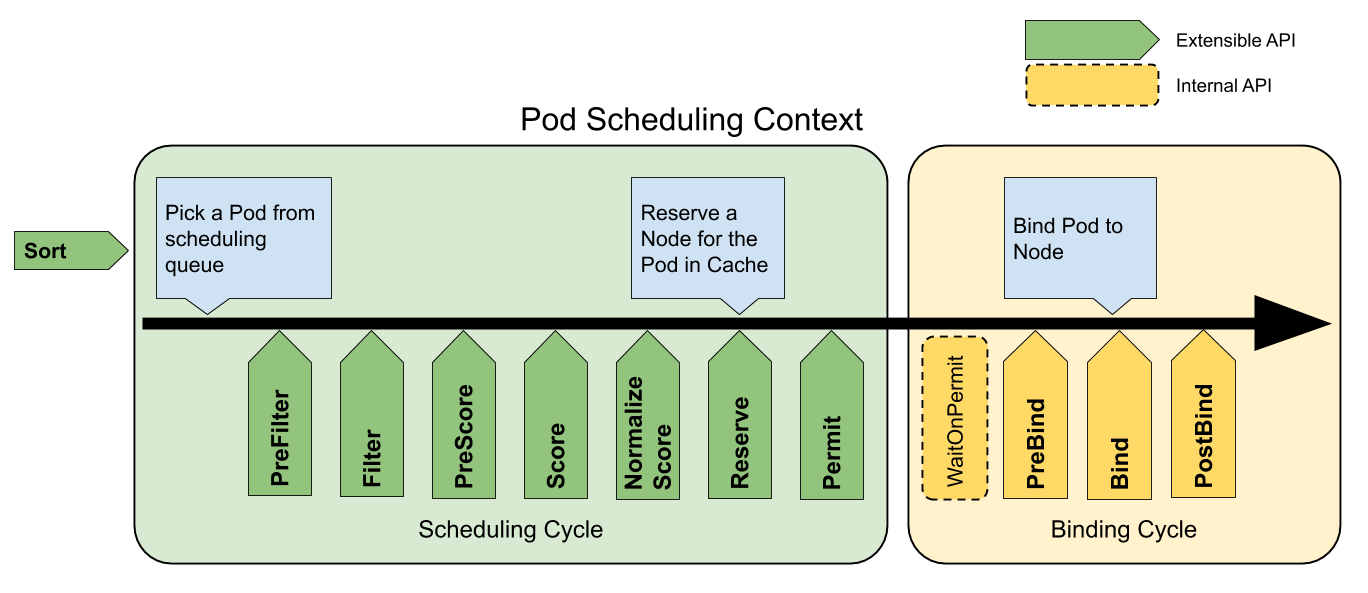
\includegraphics[width=0.80\textwidth]{k8s_scheduler}
    \bicaption{\quad k8s调度流程}{\quad k8s scheduler}
    \label{fig:k8s_scheduler}
\end{figure}

kubernetes基于标签的调度机制流程如图所示~\ref{fig:k8s_scheduler},其极强的灵活性有助于开发者应对不同应用的不同资源需求。但在节点侧,调度机制因其设计上的不灵活,往往阻碍了节点侧SLO保障机制发展。节点侧通常提供有限的调度手段,如将CPU敏感度作为标签,则nice值能够很好地实现此标签的功能,更低的nice值意味着应用能够分配到更多的时间片,从满足应用对CPU资源的需求。然而当前数据中心中应用多样,分析云场景中常见应用的监测数据,发现这些应用在资源的使用上存在较大差异,单一资源的调控难以满足节点侧调度的需求。为解决开发者的需求,内核引入了Cgroup技术,允许在CPU、Memory、Network、IO等各个子系统中细粒度的资源上调控,每一个Cgroup都可以视为一种标签,在内核的发展过程中,Cgroup与调度子系统的结合也越来越紧密。本论文希望在节点维度提供一种基于标签的节点侧调度机制,并借助节点侧在时间、资源粒度上的优势,提供更好的SLO保障。

\section{国内外相关研究}

\subsection{可观测性及劣化监测研究现状}

可观测性指通过监控、日志记录、跟踪和其他数据收集手段来描述系统的状态,从而协助理解和诊断系统的行为和性能。近年来,DevOps理念逐渐在在企业中大范围推广,可观测性作为其中的核心部分,能够解决两个主要问题。首先,在一个软件系统的生命周期中,运维是一个非常重要的部分,可观测性技术为运维提供了数据基础,帮助运维人员进行主动诊断、分析问题并追溯问题的根源,使得系统更加健壮,其次,随着软件迭代的速度越来越快,开发人员同样依赖一定的可观测性技术,来对优化结果进行评估,从而方便进一步地改进系统性能。可观测性通常随应用架构变化而发展,数据中心的早期常见的应用大多是单机服务,对进程的监控就能实现可观测性,而操作系统本身就提供了一系列的内核文件系统用于观查进程,而通过top、perf等工具就够实现进程监控。这种方式存在一些弊端,即种类繁多的指标缺乏统一的编解码格式,导致不同工具的监控难以统一分析,当前以Prometheus为主的监控技术提出Mertic格式解决了这一问题,同时统一编码方便了指标的存储、查询与分析,使得可观测性技术扩展为监控、存储、查询与分析的统一系统。云原生时代应用大多都采用微服务架构,不同于单机服务,微服务多进程、跨机器的特性是的原有的可观测性技术难以满足监控需求,2010年Google发表了Dapper\citep{sigelman2010dapper},描述了他们在微服务可观测性上的探索,并提出了分布式追踪概念,其实现原理是在请求中附加额外的span信息,并通过span之间的树形关系还原出请求在链路上的时间分布,这一工作解决了对微服务的可观测性问题,并引领出Opentracing等开源工作。日志长时间以来是应用可观测性的基本手段,日志数量大、信息复杂的特点使得相关工作通常围绕日志的存储、检索展开。当前可观测性也呈现出不同的态势。在技术上,集群监控中以kubernetes为主的管理系统开放了CNI,运行用户自定义容器网络,基于此构造出来的overlay网络能够提供网络层次更多的可观测性,节点侧则以eBPF技术为代表,使得内核能够更方便、安全地向外部应用程序提供更底层的信息。而在架构上,Opentelemetry为代表的开源项目希望将监控、日志与追踪三者结合起来,从而能够在更高层次整合不同的来源的监控信息,提供更全面的可观测性。

劣化检测通常基于一定的可观测性技术。Google在早期的数据中心中使用CPI来作为应用的性能指标[3],CPI最早用于描述微观体系结构性能,Google将其作为云环境中工作复杂的性能测量代理,应用正常运行时,CPI通常在一个小范围内波动,而当应用性能下降时,CPI会非常明显的波动,通过设定相应的阈值就能够用来监测应用的性能劣化。然而CPI并非一直都有效,Li Yi[4]等人的研究指出在低核心频率下CPI作为性能指标存在误差,并提出了RCPI进行修正。近年来AI技术不断发展,可观测性系统获取了大量的时序数据,同时观查指标能够发现存在一定的规律性,这使得通过AI技术分析监测数据,从而提前预测到SLO的破坏并做出行动成为可能\citep{qiu2020firm, zhou2022aquatope, wang2022deepscaling, gan2021sage}。FIRM\citep{qiu2020firm}中以kubenetes集群为背景,设计了一个两级机器学习模型来识别SLO的破坏,并在实验中取得了相当显著的效果,Di Wu\citep{wu2020data}则提出了一种数据特性感知潜在因素(DCALF)模型来实现高精度的QoS预测,能够依据不同QoS数据的特性来分别的进行预测。尽管AI技术在集群维度取得了显著的效果,但是由于其数据量大、计算复杂的特点,在宽容度较低的节点侧难以进行部署。


\subsection{基于资源划分的调度研究现状}

资源不足通常会导致应用的性能劣化,而不同的应用对于不同资源的需求存在差异,因此能够以多种资源为目标设计调度机制\citep{delimitrou2014quasar, lo2015heracles}。可观测性技术能够提供系统的资源状况,基于资源划分的调度要求系统中存在或能够通过一些技术构造出资源的隔离域,在集群维度,独立的节点本身就是一种隔离域,而基于机架、网络等因素划分的节点群就构成了更上层的隔离域,而在节点则能够通过Cgroup、Intel RDT等技术构造更细粒度的隔离域。劣化监测能够发现SLO的破坏并触发调度过程,越精确的监测机制能够带来更好的效果。而在基于资源划分的调度过程中,一般是在隔离域间移动应用,或是调整应用所处隔离域的资源划分,来避免资源不足的情况,从而保证应用的SLO。

集群维度中,资源划分通常是静态的,因此调度过程通常以选择合适放置的节点为目标,实际上是在解决一种装箱问题。集群维度中导致应用资源不足的原因通常是不合适的放置或是不及时的调度,使得节点上竞争资源过载,引发应用SLO的破坏。微软Azure是世界上最大的云服务平台之一,其数据中心数量庞大,且横跨多个地域,在组织架构上也分为多个层次,为放置策略的设计带来较大的困难,Protean\citep{hadary2020protean}是Azure中对虚拟机放置问题的解决方案,通过多级的分配规则来分层处理以地域、数据中心、机架上的虚拟机放置,来实现充分的资源利用。

\begin{figure}[!htbp]
    \centering
    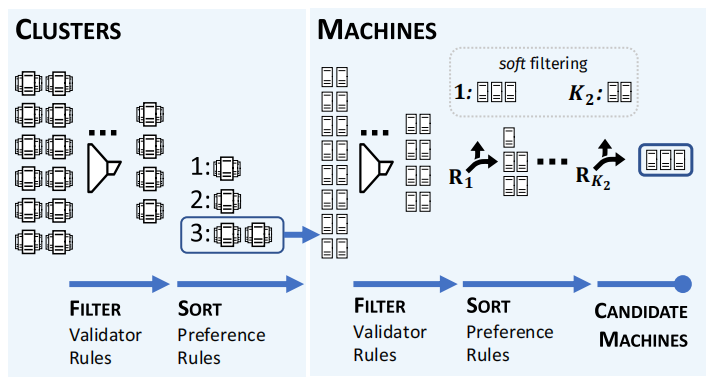
\includegraphics[width=0.80\textwidth]{protean_location}
    \bicaption{\quad Protean放置流程}{\quad protean location}
    \label{fig:protean_location}
\end{figure}

节点视角中,问题则更加复杂,这主要有两个原因,首先,应用资源需求是动态变化的,而调度只能基于某一时刻的资源划分情况,当应用资源需求变化时,先前的决策就可能变得不合理从而引发节点内资源竞争,实际云场景下,服务型应用通常都具有资源需求随负载而变化的特点,而为解决这样的问题,就要求调度器必须尽可能迅速地监测劣化情况,并及时做出决策。其次,应用的资源需求是多样的,而绝大多数节点侧调度都以CPU时间片为粒度,在当前数据中心服务器片上资源越来越丰富的背景下,这种面向单一资源的调度机制,难以应对其他资源上的竞争,Parties\citep{chen2019parties}则提供了一种多资源调度的实践,其调度算法考虑到了应用不同的资源需求及不同资源之间的置换关系,能够在保证总体利用率的前提下尽可能的保证应用性能。

基于资源划分的调度效果依赖可观测性与调度机制的结合程度,集群调度提供了相对统一的接口,两者结合非常成熟,并且集群调度相对宽容,这就大大简化了调度器的设计难度,通常效果也相对较好。而在节点侧则存在诸多问题,由于软件环境复杂,可观测性通常与调度机制相对割裂,因此调度器设计中必须充分考虑,这无疑会增加调度器的设计难度,其次,对于用户态的调度器而言,由于节点侧要求低延时高频率的调度,因此在可观测性应当避免较为复杂的机制,但这可能会导致观测的精度降低,同时,以进程为目标的调度依赖内核提供的接口,而在当前内核的实现中,这些接口的作用更多是指导内核调度,因此在机制实现上并不直接,从而影响调度的精度,并且在硬件机制上,尽管Intel RDT技术提供了对LLC及内存带宽的有限隔离[9],但其生效延迟会同样影响到调度精度,而无论观测还是调度的精度,都最终会影响到调度效果,这就使得基于资源划分的调度机制在节点侧上的表现并不优异。

\subsection{内核调度及任务调度研究现状}

基于资源划分的调度在节点侧推动种种困难,使得人们对于节点侧调度的思考回归到任务调度上\citep{fried2020caladan, ousterhout2019shenango, prekas2017zygos}。任务调度通常依赖一个一种运行时,来提供任务的上下文保存、中止与恢复等,实际上是控制任务对于CPU资源的使用,而通常以CPU为核心编程,资源请求都会随应用在CPU上的运行而产生,以CPU为粒度的调度虽较粗,但存在其可行性。

节点侧的内核是进程的运行时,内核提供了完全公平调度器、实时调度器、截止日期调度器、闲置调度器等来满足用户在不同使用场景下对进程进行调度的需求。其中完全公平调度器应用较为广泛[10],同时完全公平调度器也是典型的基于CPU time的调度器。完全公平调度器的调度目标是让所有进程都能够分配到相同的时间片数量,同时允许用户设置优先级来让高优先级的任务获得更多的时间片,具体实现中调度器会为每一个进程维护一个时间记账信息,同时使用红黑树组织运行队列中的进程,在每个时钟中断到来时更新进程时间记账,并从红黑树中取得vruntime最小的进程执行。完全公平调度器在多数场景下都能有效地保障节点的吞吐,因此也长期作为内核的默认调度器,但是完全公平调度器也存在不足之处。第一,完全公平调度器虽然能为优先级更高的进程分配更多的时间片,但无法做到更快地为优先级高的进程分配时间片,这因为完全公平调度器机制上的时间片粒度对所有进程都是相同的。数据中心常见的应用可分为LC与BE应用,其中LC应用对延迟较敏感,减小CFS调度器的时间片能保障其QoS要求,但这回引入多的上下文切换开销,对于需要持续运行的BE应用而言就会受到较大的性能影响,因此在6.6版本的内核中选择将EEVDF作为默认调度器替换了CFS调度器。EEVDF调度器同样是基于CPU time的调度器,其为每个进程设置了一个截止日期,并在每次调度时选择最早截至日期的进程\citep{stoica1995earliest},与CFS不同之处在于,EEVDF中加入的 latency nice 特性,允许分配给应用更小时间片来让其给更快地获得CPU time。第二,无论CFS调度器还是EEVDF调度器,都只基于CPU time进行调度,这对于单CPU上调度来说无可厚非,但对于SMP系统而言,仅基于CPU time的调度就容易产生问题。

内核基于SMP系统的CPU拓扑构建调度域,并基于此进行负载均衡,但需要注意的是,CPU拓扑并非是完全的隔离域,每层调度域之间实际上都存在一定的竞争。逻辑核上通过分时复用将两个进程在时间域上隔离,这几乎隔离了所有资源,然而现代微体系结构并没有严格保证这种隔离,研究发现,当前一个任务允许AVX512指令时,出于功耗的考量,CPU会降频以避免过热,并在AVX512指令执行完毕之后恢复频率,然而这个恢复过程并非是立刻完成的,而需要一定的时间\citep{gottschlag2020avx},假设在此期间发生了任务的切换,则显然下一个任务的执行就会受到影响。对于Hyperthread上的兄弟核而言,除频率之外还会受到Cache及运算器竞争的影响,对于一些指令并行度高的任务而言,这种竞争就会使得其性能下降。对于Numa上的所有核心而言,由于LLC与内存带宽的共享,容易发生“吵闹邻居”的现象,而这很难通过CPU time进行调节。对于相同Socket上的核心而言,由于TDP的限制,因此功耗也会称为竞争的目标,这体现在CPU频率上,当前CPU支持 Turbo boost 功能,允许在CPU整体负载低时,允许部分核心超越其基准频率允许来达到更快的执行速度,这会导致Socket内,相互独立的CPU会因为整体的负载强度导致允许频率被间接的影响,从而影响 CPU time 的精度。Elfen\citep{yang2016elfen}尝试通过修改内核调度器,提供兄弟核心负载监测与快速的资源出让来应对Hyperthread上的资源竞争问题,而Gottschlag\citep{gottschlag2020avx}则尝试通过补偿受害者进程的CPU time 来提升内核调度器的公平性,从而解决Turbo boost所导致的Socket上的功耗竞争问题。

节点侧软件环境的复杂性也体现在任务运行时之间的相互干扰,如对于一个Go程序而言,协程受到运行时的调度,而运行时本身又作为一个进程运行在内核之上,通常下层运行时无法感知上层运行时的调度决策,因此就容易出现协程被Go运行时调度运行,而Go运行时却被内核调度下去,导致应当执行的任务没有被执行的情况出现。因此在节点侧的调度通常都会避免复杂化的运行时层级,而选择对已有层级运行时进行修改,如Elfen就是在内核层对调度器进行的修改,这种做法既能够直接在内核态获取大量的观测信息,也能够避免跨层次的运行时所产生的调度噪声。Caladan\citep{fried2020caladan}做法则是在内核运行时之上实现了一个用户态的运行时,并通过DPDK、SPDK将IO都在用户态进行,同时关闭内核抢占来去尽可能地规避内核调度器的噪声。这种做法将调度完全置于用户态,规避了在内核进行开发的种种限制,使得Caladan能够设计更复杂的调度策略,利用节点侧更细的调度频率与资源使用感知,实现更好的任务调度。

\section{论文的研究内容}

本文的研究内容从三个方面进行展开,首先,课题选择云场景中场景的应用进行离线画像分析,获取其资源使用特征及资源敏感程度等信息,并在此基础上进一步聚类分析获取不同资源的关键性能指标与敏感度类型,构造基本指标系统。其次,课题预期在节点侧设计一种基于标签的调度机制,根据应用所携带的不同标签,及时感知此标签所关联的关键指标变化,并触发对应的调度策略。最后,课题预期针对不同的标签设计差异化的调度策略,满足不同应用对于不同资源的需求,同时考虑多种标签应用共置的场景,能够在保证应用 QoS 的前提下,尽可能地提升资源利用率。

\subsection{典型应用画像与混部分析}

预期完成一个指标采集、分析系统与各个应用的画像分析。指标采集系统能够从系统、应用等各个维度采集信息,分析系统则能够对时序数据进行一定的处理并挖掘呈现出关键信息。应用画像提供应用在资源使用倾向、干扰敏感度上的信息,分析每个应用在性能上的关键指标,分析关键指标变化的核心因素。同时提供在不同应用之间横向对比,挖掘出共性的聚类情况,并对关联性进行解释,最后从画像分析结果中构建基本的指标系统。

\subsection{运行时可变内核调度框架实现}

预期提供一套节点侧基于标签的调度器。调度器能够从内核的各个子系统中中获取丰富的指标信息,并能够将其转化为不同子系统上的标签。同时调度器提供了调度进程的关键功能,如启动、关闭、迁移等,并暴漏给外部进行调用。最后还提供一套编程框架,基于调度器暴漏的接口,允许自定义调度策略。

\subsection{资源感知调度系统实现}

预期提供不同的QoS保障策略,来应对不同应用的资源使用需求。策略基于调度器提供的框架设计,能够通过标签感知应用对不同资源的敏感度,并调度时考虑应用本身以及其所处的隔离域上的资源使用情况,在保障应用的QoS的同时,还能够提升整体资源的利用率。

\section{论文结构安排}
